\documentclass[conference]{IEEEtran}
\IEEEoverridecommandlockouts
% The preceding line is only needed to identify funding in the first footnote. If that is unneeded, please comment it out.
%Template version as of 6/27/2024

\usepackage[colorlinks=true, linkcolor=black, citecolor=blue, urlcolor=blue]{hyperref}

\usepackage{cite}
\usepackage{amsmath,amssymb,amsfonts}
\usepackage{algorithmic}
\usepackage{graphicx}
\usepackage{textcomp}
\usepackage{xcolor}
\def\BibTeX{{\rm B\kern-.05em{\sc i\kern-.025em b}\kern-.08em
	T\kern-.1667em\lower.7ex\hbox{E}\kern-.125emX}}
\begin{document}

%\title{Conference Paper Title*\\
	%{\footnotesize \textsuperscript{*}Note: Sub-titles are not captured for https://ieeexplore.ieee.org  and
		%should not be used}
	%\thanks{Identify applicable funding agency here. If none, delete this.}
	%}
%
%\author{\IEEEauthorblockN{1\textsuperscript{st} Given Name Surname}
	%\IEEEauthorblockA{\textit{dept. name of organization (of Aff.)} \\
		%\textit{name of organization (of Aff.)}\\
		%City, Country \\
		%email address or ORCID}
	%\and
	%\IEEEauthorblockN{2\textsuperscript{nd} Given Name Surname}
	%\IEEEauthorblockA{\textit{dept. name of organization (of Aff.)} \\
		%\textit{name of organization (of Aff.)}\\
		%City, Country \\
		%email address or ORCID}
	%\and
	%\IEEEauthorblockN{3\textsuperscript{rd} Given Name Surname}
	%\IEEEauthorblockA{\textit{dept. name of organization (of Aff.)} \\
		%\textit{name of organization (of Aff.)}\\
		%City, Country \\
		%email address or ORCID}
	%\and
	%\IEEEauthorblockN{4\textsuperscript{th} Given Name Surname}
	%\IEEEauthorblockA{\textit{dept. name of organization (of Aff.)} \\
		%\textit{name of organization (of Aff.)}\\
		%City, Country \\
		%email address or ORCID}
	%\and
	%\IEEEauthorblockN{5\textsuperscript{th} Given Name Surname}
	%\IEEEauthorblockA{\textit{dept. name of organization (of Aff.)} \\
		%\textit{name of organization (of Aff.)}\\
		%City, Country \\
		%email address or ORCID}
	%\and
	%\IEEEauthorblockN{6\textsuperscript{th} Given Name Surname}
	%\IEEEauthorblockA{\textit{dept. name of organization (of Aff.)} \\
		%\textit{name of organization (of Aff.)}\\
		%City, Country \\
		%email address or ORCID}
	%}

\title{Deriving IT Strategies from Times Higher Education Rank}
 \author{\textbf{[Hidden for double-blind review]}}
%\author{\IEEEauthorblockN{
%		Alfa Yohannis%\IEEEauthorrefmark{1}
%		\IEEEauthorrefmark{2},
%		Master Edison Siregar%\IEEEauthorrefmark{1}%\IEEEauthorrefmark{3}
%	}
%	\IEEEauthorblockA{
%		% \IEEEauthorrefmark{1}
%		Hidden for Double-blind Review
%		Department of Informatics\\
%		Pradita University, Tangerang, Indonesia\\
%		\IEEEauthorrefmark{2}alfa.ryano@pradita.ac.id}
%	% 	% \IEEEauthorblockA{
%		% 	% 	\IEEEauthorrefmark{2}Department of Computer Science\\
%		% 	% 	University of York, York, United Kingdom}
%}

\newcommand{\al}[1]{{\textbf{\color{blue} Al: #1}}}

\maketitle

\begin{abstract}
	This study explores the correlations among key metrics from the Times Higher Education (THE) rankings over a 10-year period to derive actionable IT strategies for universities. Using rigorous analysis, including Spearman's Rank Correlation, the research identifies the most influential variables affecting institutional performance, such as research and teaching scores, citations, and international outlook. The findings underscore the importance of aligning IT investments with these critical areas to enhance institutional rankings and competitiveness. Based on the analysis, targeted IT strategies are recommended to support the performance of higher education institutions based on the influential variables.
\end{abstract}

\begin{IEEEkeywords}
	IT Strategy, Higher Education, Times Higher Education Rankings, Correlation Analysis
\end{IEEEkeywords}


\section{Introduction}


The role of Information Technology (IT) strategy has become increasingly significant across various sectors, including Higher Education \cite{hashim2021higher}. In an era where digital transformation drives innovation, IT strategies are crucial for achieving institutional goals, enhancing operational efficiency, and improving the quality of services provided \cite{rahmadi2024research}. Within the context of Higher Education, these strategies are vital for ensuring that institutions remain competitive in an increasingly dynamic academic environment \cite{fernandez2023digital}.

IT strategies in Higher Education are often developed through diverse methodologies, including strategic alignment with institutional goals, benchmarking against peer institutions, and leveraging frameworks such as enterprise architecture \cite{bianchi2023it}. These approaches aim to optimise the utilisation of technology to support academic excellence, enhance research outputs, and improve student engagement \cite{digitalsystems2022strategy}.

Moreover, global ranking systems, such as those provided by \textit{Times Higher Education (THE)}, introduce variables that significantly influence universities' positions in these rankings \cite{times2023methodology}. Factors such as research output, teaching quality, industry collaboration, and international outlook play a pivotal role in determining an institution’s rank \cite{times2022rankings}. By analysing the relationships between these variables, it becomes possible to identify which aspects should be prioritised within IT strategies to maximise their impact on institutional performance.



This study aims to explore the relationships among key variables highlighted by \textit{Times Higher Education (THE)} and how these insights can inform the development of effective IT strategies tailored to the needs of Higher Education institutions. Through an analysis of the correlations between these variables, patterns and dependencies are identified, highlighting critical areas of focus for IT investments. Based on this analysis, a set of IT strategies is proposed to specifically target improvements in the variables most significant to universities' performance.

This paper is structured into several sections. The Introduction highlights the significance of IT strategy in Higher Education, while the Related Work reviews studies on deriving such strategies, focusing on methodologies and the role of \textit{Times Higher Education} rankings. The Methodology describes the analysis of these rankings' variables. The Results and Discussion present key findings, followed by IT Strategy Recommendations offering actionable insights. Finally, the Conclusion and Future Work summarise the study's contributions and suggest future research directions.


\section{Literature Review}
\label{sec:literature_review}

The development of an Information Technology (IT) strategy is a critical process that aligns technology initiatives with organisational objectives. Various frameworks and methodologies have been proposed in the literature to aid this alignment, ensuring that IT contributes to achieving competitive advantage and operational efficiency.

\subsection{Frameworks for IT Strategy Development}

Drechsler and Weißschädel \cite{drechsler2018framework} proposed a framework tailored for small and medium enterprises (SMEs) to develop IT strategies. Their approach integrates theoretical foundations with empirical validation, ensuring practical relevance for organisations with limited resources. The framework emphasises iterative processes, allowing organisations to adapt their strategies dynamically as they grow and encounter new challenges.

El Alami and Belemlih \cite{elalami2021digital} explored the integration of IT governance and management frameworks, such as COBIT, to formulate a digital strategy. Their study highlights the importance of combining existing best practices to address emerging digital transformation needs. By focusing on governance, organisations can align IT objectives with overall business strategies effectively.

De Haes and Van Grembergen \cite{dehaes2009governance} emphasised the role of IT governance frameworks in supporting IT strategy development. They discussed the use of maturity models to assess and improve IT alignment with organisational goals. Their work also highlights the importance of executive-level involvement in IT decision-making processes.

\subsection{Alignment with Organisational Objectives}

Adama et al. \cite{adama2024alignment} examined theoretical frameworks that support the alignment of IT and business strategies to achieve sustained competitive advantage. They argue that IT strategy should not only support current business operations but also anticipate future market demands and technological advancements. This forward-looking approach ensures that IT remains a strategic asset rather than a mere operational tool.

Putra et al. \cite{putra2022trends} conducted a systematic review of IT strategy implementation trends across various sectors. Their findings underscore the challenges organisations face in aligning IT strategies with broader organisational objectives. Key barriers include resource constraints, resistance to change, and the complexity of integrating legacy systems with modern technologies.


\subsection{Challenges in IT Strategy Formulation}

Rahmadi \cite{rahmadi2024research} identified digital transformation as a key driver of IT strategy development. However, he also noted that many organisations struggle to keep pace with technological advancements. His research highlights the need for adaptive strategies that can evolve with changing market conditions and technological landscapes.

Fernández et al. \cite{fernandez2023digital} conducted a multivocal literature review of digital transformation initiatives in higher education. They emphasised the importance of stakeholder engagement in IT strategy development, noting that successful strategies often involve collaboration between IT departments, academic staff, and administrative leaders.

\subsection{Emerging Trends and Future Directions}

The increasing complexity of IT environments has led to the adoption of more sophisticated tools and methodologies for strategy development. For instance, machine learning and predictive analytics are now being used to forecast the impact of IT investments on organisational performance. These technologies enable more informed decision-making and greater agility in responding to market changes \cite{digitalsystems2022strategy}.


\subsection{Use of Rankings and Performance Metrics}

Performance metrics\footnote{The terms `metrics' and `variables' are used interchangeably.} play a pivotal role in shaping IT strategies, particularly in higher education institutions. Rankings such as those provided by Times Higher Education (THE) emphasize variables such as research output, teaching quality, and international collaboration as critical factors influencing university competitiveness. Integrating these metrics into IT strategies enables institutions to align their technological initiatives with objectives that enhance their global standing \cite{times2023methodology}.

Da Silva and Santos \cite{dasilva2014cobit} examined IT governance frameworks and their application in strategic planning, demonstrating that metrics derived from ranking systems like THE can serve as benchmarks for prioritising IT investments. This approach ensures that IT initiatives directly contribute to improving institutional rankings and overall performance.

Further exploration of the relationship between ranking metrics and strategic planning is provided by Uslu \cite{uslu2020university}, who analysed key indicators from international university rankings, including THE. Uslu's findings reveal how metrics such as research output, teaching quality, and international collaboration can inform institutional strategies aimed at enhancing competitiveness. By understanding the weight and impact of these indicators, universities can craft IT strategies that target specific areas for improvement, directly contributing to enhanced rankings.

A complementary perspective is offered by a study on university competitiveness through data analytics \cite{analytics2022competitiveness}, which proposed predictive models to assist universities in improving their performance in rankings like THE. These models leverage historical ranking data and institutional metrics to identify areas requiring focused improvement. The study underscores the importance of IT in enabling data-driven decision-making and strategic planning, ensuring that technology investments are directed towards metrics with the highest potential impact.

Although the direct linkage between THE metrics and IT strategy development is not always explicit, these studies collectively provide actionable insights. Universities can harness IT to implement strategies that enhance performance in areas such as research output, teaching excellence, and global collaboration—key drivers of improved ranking outcomes.

This research builds on these foundations by taking a unique approach. It examines THE metrics and variables over a longitudinal period of 10 or more years, providing a deeper understanding of their correlations and influence on institutional rankings. By identifying the most impactful variables, this study offers a framework for developing IT strategies that specifically address these critical areas. Such targeted strategies ensure that IT investments are optimally aligned with institutional objectives, maximising their impact on performance and ranking outcomes.


\section{Methodology}
\label{sec:methodology}

The research was performed quantitatively, with data collected through web scrapping. Python scripts were written to process, analyse, and visualise the collected data using its various libraries. 

\subsection{Data Collection and Cleaning}

The data scrapping was achieved by collecting universities' ranks and rank factors by scrapping scores from 2013 to 2023 in the Times Higher Education (THE) website \cite{the2024} and combining it with the data of university ranks obtained from Kaggle \cite{ONeil_2020}\footnote{The contribution of this dataset was minimal.}, producing more than 11-year data span with 711 universities involved. 

After collecting the necessary data, it underwent several data-cleaning steps to ensure it was ready for analysis. First, empty numeric values were filled using linear estimation, logarithmic estimation, etc., based on the coefficient of determination $R^{2}$ to estimate the missing values. The filled values were then normalised and added as a new column to the dataset. Secondly, empty non-numeric values were filled with `n/a' to help handle missing non-numeric values in the following steps.

Finally, unnecessary columns were removed to streamline the dataset, and only several columns were used in the analysis as variables. These variables were overall score, rank, research score, teaching score, citations score, intl students, international outlook score, student staff ratio, industry income score, number students, year. 

\subsection{Data Analysis}

Correlations were calculated between the variables. The analysis assessed the strength of the relationships using correlation coefficients, along with their statistical significance. Spearman's Rank Correlation Coefficient \cite{spearman1904general} was employed to ensure the robustness of the results, as it does not assume normality in the data distribution. The significance of the correlations was evaluated to determine whether the observed relationships were likely to have occurred by chance. A graph chart was used to help comprehend the data, that nodes represented the variables of THE and edges were the correlations between them. 

\begin{figure*}[t]
	\centering
	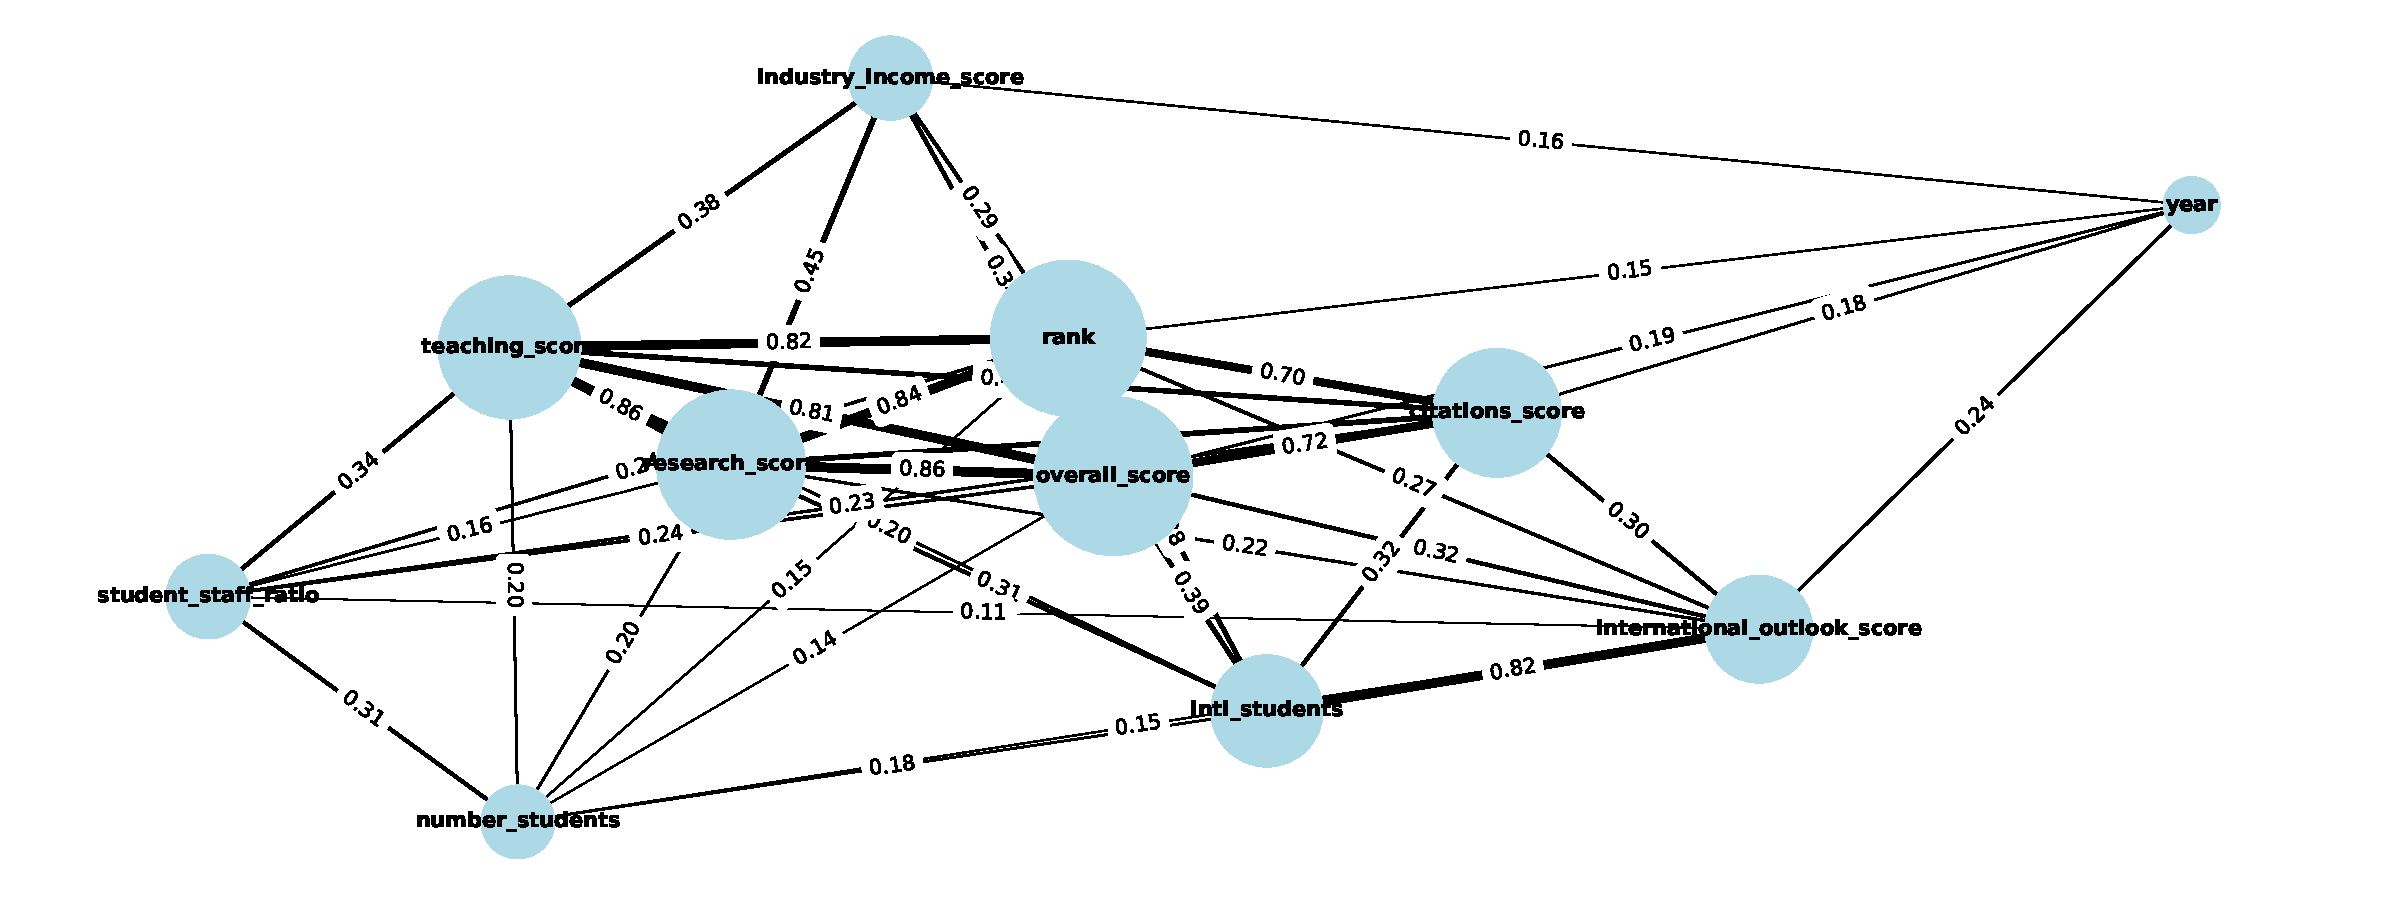
\includegraphics[width=\linewidth]{figures/correlation_graph.pdf}
	\caption{Correlation graph between the variables of Times Higher Education Rank. Correlations with }
	\label{fig:graf_citation}
\end{figure*}

\section{Results and Discussion}
This section examines the correlations among THE variables, including international outlook score, rank, citations score, overall score, industry income score, international students, research score, number of students, student-to-staff ratio, and teaching score. A summary of these correlations is presented in Fig. \ref{fig:graf_citation}. The graph highlights only significant correlations with a strength greater than 0.1. Additionally, the diameter of each node represents the variable's overall influence, calculated as the sum of its correlations with other variables.


\subsection{Analysis of Correlations with Overall Score}

The correlation analysis highlights key factors associated with the \textit{overall score}, emphasizing its role as a comprehensive measure of institutional performance (Table \ref{tab:correlation_overall}). Among the variables examined, the \textit{rank} ($r = -0.89$), \textit{research score} ($r = 0.86$), and \textit{teaching score} ($r = 0.81$) exhibit the strongest correlations. The strong negative correlation with \textit{rank} underscores the critical relationship between overall institutional performance and competitive standings. Similarly, the high positive correlations with \textit{research score} and \textit{teaching score} highlight the importance of academic and research excellence in achieving higher overall scores.

Moderate correlations are observed for \textit{citations score} ($r = 0.72$), \textit{international students} ($r = 0.39$), \textit{industry income score} ($r = 0.34$), and \textit{international outlook score} ($r = 0.32$). These findings suggest that impactful research, global engagement, and industry collaborations substantially contribute to shaping the overall score.

Weaker correlations include \textit{student-to-staff ratio} ($r = -0.24$), \textit{year} ($r = 0.19$), and \textit{number of students} ($r = 0.14$). While these variables show limited direct influence on the overall score, maintaining favorable ratios and engaging large student populations remain important for broader institutional objectives.

\begin{table}[h!]
	\centering
	\caption{Correlation Analysis Results for \textbf{Overall} Score}
	\label{tab:correlation_overall}
	\begin{tabular}{|l|r|r|}
		\hline
		\textbf{Variable} & \textbf{Corr. ($r$)} & \textbf{p-value} \\
		\hline
		Rank & -0.89 & 0.00\textsuperscript{***} \\
		Research Score & 0.86 & 0.00\textsuperscript{***} \\
		Teaching Score & 0.81 & 0.00\textsuperscript{***} \\
		Citations Score & 0.72 & 0.00\textsuperscript{***} \\
		International Students & 0.39 & 0.00\textsuperscript{***} \\
		Industry Income Score & 0.34 & 0.00\textsuperscript{***} \\
		International Outlook Score & 0.32 & 0.00\textsuperscript{***} \\
		Student-to-Staff Ratio & -0.24 & 0.00\textsuperscript{***} \\
		Year & 0.19 & 0.00\textsuperscript{***} \\
		Number of Students & 0.14 & 0.00\textsuperscript{***} \\
		\hline
	\end{tabular}
\end{table}



\subsection{Analysis of Correlations with Rank}

The correlation analysis highlights key determinants influencing institutional rankings (Table \ref{tab:correlation_rank}). Among the examined variables, the \textit{overall score}, \textit{research score}, \textit{teaching score}, and \textit{citations score} exhibit the strongest negative correlations, underscoring their significant impact on rank. The \textit{overall score} ($r = -0.89$) and \textit{research score} ($r = -0.84$) emerge as the most influential factors, emphasizing their critical roles in driving institutional performance and competitiveness.

Moderate negative correlations are observed for \textit{teaching score} ($r = -0.82$), \textit{citations score} ($r = -0.70$), and \textit{international students} ($r = -0.38$), highlighting the importance of academic quality, research impact, and global engagement in shaping rankings. Weaker negative correlations are found for \textit{industry income score} ($r = -0.29$) and \textit{international outlook score} ($r = -0.27$), reflecting their secondary influence on institutional rankings.

Positive correlations are observed for \textit{student-to-staff ratio} ($r = 0.24$) and \textit{year} ($r = 0.15$), suggesting that less favorable staff ratios and newer data are weakly associated with poorer rankings. The \textit{number of students} ($r = -0.15$, $p = 0.00$) demonstrates a small but significant negative relationship, indicating limited influence on rank outcomes.

These results reinforce the centrality of performance-driven metrics, particularly those related to research and teaching quality, in shaping institutional rankings. While internationalization factors add further depth, their impact is relatively modest compared to core academic indicators.

\begin{table}[h!]
	\centering
	\caption{Correlation Analysis Results for Institutional \textbf{Rank}}
	\label{tab:correlation_rank}
	\begin{tabular}{|l|r|r|}
		\hline
		\textbf{Variable} & \textbf{Corr. ($r$)} & \textbf{p-value} \\
		\hline
		Overall Score & -0.89 & 0.00\textsuperscript{***} \\
		Research Score & -0.84 & 0.00\textsuperscript{***} \\
		Teaching Score & -0.82 & 0.00\textsuperscript{***} \\
		Citations Score & -0.70 & 0.00\textsuperscript{***} \\
		International Students & -0.38 & 0.00\textsuperscript{***} \\
		Industry Income Score & -0.29 & 0.00\textsuperscript{***} \\
		International Outlook Score & -0.27 & 0.00\textsuperscript{***} \\
		Student-to-Staff Ratio & 0.24 & 0.00\textsuperscript{***} \\
		Year & 0.15 & 0.00\textsuperscript{***} \\
		Number of Students & -0.15 & 0.00\textsuperscript{***} \\
		\hline
	\end{tabular}
\end{table}


\subsection{Analysis of Correlations with Research Score}

The correlation analysis highlights critical factors contributing to the \textit{research score}, emphasizing its central role in institutional performance (Table \ref{tab:correlation_research}). Among the examined variables, the \textit{overall score} ($r = 0.86$) and \textit{teaching score} ($r = 0.86$) exhibit the strongest positive correlations, underscoring their close alignment with research activities. Enhancing both teaching and overall institutional quality directly supports improvements in research performance.

The \textit{rank} ($r = -0.84$) demonstrates a strong negative correlation, reaffirming the inverse relationship where higher research scores correspond to better rankings (lower numerical rank values). This finding underscores the pivotal role of research excellence in achieving competitive standings.

Moderate correlations are observed for \textit{industry income score} ($r = 0.45$), \textit{citations score} ($r = 0.45$), and \textit{international students} ($r = 0.31$). These results suggest that impactful research outputs, industry partnerships, and global engagement significantly influence research scores. The \textit{international outlook score} ($r = 0.22$) also reflects the contribution of internationalization, though to a lesser extent.

Weaker correlations include \textit{number of students} ($r = 0.20$), \textit{student-to-staff ratio} ($r = -0.16$), and \textit{year} ($r = 0.08$). While these metrics exhibit limited direct impact on research performance, optimizing these factors may still provide ancillary benefits to institutional quality.

\begin{table}[h!]
	\centering
	\caption{Correlation Analysis Results for \textbf{Research} Score}
	\label{tab:correlation_research}
	\begin{tabular}{|l|r|r|}
		\hline
		\textbf{Variable} & \textbf{Corr. ($r$)} & \textbf{p-value} \\
		\hline
		Overall Score & 0.86 & 0.00\textsuperscript{***} \\
		Teaching Score & 0.86 & 0.00\textsuperscript{***} \\
		Rank & -0.84 & 0.00\textsuperscript{***} \\
		Industry Income Score & 0.45 & 0.00\textsuperscript{***} \\
		Citations Score & 0.45 & 0.00\textsuperscript{***} \\
		International Students & 0.31 & 0.00\textsuperscript{***} \\
		International Outlook Score & 0.22 & 0.00\textsuperscript{***} \\
		Number of Students & 0.20 & 0.00\textsuperscript{***} \\
		Student-to-Staff Ratio & -0.16 & 0.00\textsuperscript{***} \\
		Year & 0.08 & 0.00\textsuperscript{***} \\
		\hline
	\end{tabular}
\end{table}

\subsection{Analysis of Correlations with Teaching Score}

The correlation analysis highlights key factors contributing to the \textit{teaching score}, emphasizing its critical role in institutional performance (Table \ref{tab:correlation_teaching}). Among the examined variables, the \textit{research score} ($r = 0.86$), \textit{rank} ($r = -0.82$), and \textit{overall score} ($r = 0.81$) exhibit the strongest correlations. The positive correlations with \textit{research score} and \textit{overall score} underscore the alignment of teaching excellence with broader institutional quality and academic outputs. Conversely, the strong negative correlation with \textit{rank} highlights the inverse relationship, where higher teaching scores correspond to better rankings (lower numerical rank values).

Moderate correlations are observed for \textit{citations score} ($r = 0.43$), \textit{industry income score} ($r = 0.38$), and \textit{student-to-staff ratio} ($r = -0.34$). These findings indicate that impactful research, robust industry collaborations, and favorable staff-to-student ratios significantly influence teaching quality.

Weaker correlations include \textit{international students} ($r = 0.20$), \textit{number of students} ($r = 0.20$), \textit{international outlook score} ($r = 0.03$), and \textit{year} ($r = 0.02$). While these variables exhibit limited direct influence on teaching performance, they may contribute indirectly by shaping the broader institutional environment.

\begin{table}[h!]
	\centering
	\caption{Correlation Analysis Results for \textbf{Teaching} Score}
	\label{tab:correlation_teaching}
	\begin{tabular}{|l|r|r|}
		\hline
		\textbf{Variable} & \textbf{Corr. ($r$)} & \textbf{p-value} \\
		\hline
		Research Score & 0.86 & 0.00\textsuperscript{***} \\
		Rank & -0.82 & 0.00\textsuperscript{***} \\
		Overall Score & 0.81 & 0.00\textsuperscript{***} \\
		Citations Score & 0.43 & 0.00\textsuperscript{***} \\
		Industry Income Score & 0.38 & 0.00\textsuperscript{***} \\
		Student-to-Staff Ratio & -0.34 & 0.00\textsuperscript{***} \\
		International Students & 0.20 & 0.00\textsuperscript{***} \\
		Number of Students & 0.20 & 0.00\textsuperscript{***} \\
		International Outlook Score & 0.03 & 0.07 * \\
		Year & 0.02 & 0.28 \\
		\hline
	\end{tabular}
\end{table}


\subsection{Analysis of Correlations with Citations Score}

The correlation analysis identifies key factors associated with the \textit{citations score}, highlighting its significance as a measure of research impact (Table \ref{tab:correlation_citations}). Among the variables examined, the \textit{overall score} ($r = 0.72$) exhibits the strongest positive correlation, underscoring the alignment between high overall institutional performance and research impact through citations. The \textit{rank} ($r = -0.70$) shows a strong negative correlation, emphasizing the critical role of citations in improving institutional rankings (lower numerical rank values).

Moderate positive correlations are observed for \textit{research score} ($r = 0.45$), \textit{teaching score} ($r = 0.43$), \textit{international students} ($r = 0.32$), and \textit{international outlook score} ($r = 0.30$). These findings indicate that impactful research, quality teaching, and global engagement significantly contribute to citation performance.

Weaker correlations include \textit{student-to-staff ratio} ($r = -0.23$) and \textit{year} ($r = 0.18$), suggesting limited but notable influence on citations. The \textit{industry income score} ($r = 0.05$) demonstrates a weak positive correlation, while the \textit{number of students} ($r = 0.02$, $p = 0.24$) shows a negligible and statistically insignificant relationship, highlighting their minimal relevance to citations.

\begin{table}[h!]
	\centering
	\caption{Correlation Analysis Results for \textbf{Citations} Score}
	\label{tab:correlation_citations}
	\begin{tabular}{|l|r|r|}
		\hline
		\textbf{Variable} & \textbf{Corr. ($r$)} & \textbf{p-value} \\
		\hline
		Overall Score & 0.72 & 0.00\textsuperscript{***} \\
		Rank & -0.70 & 0.00\textsuperscript{***} \\
		Research Score & 0.45 & 0.00\textsuperscript{***} \\
		Teaching Score & 0.43 & 0.00\textsuperscript{***} \\
		International Students & 0.32 & 0.00\textsuperscript{***} \\
		International Outlook Score & 0.30 & 0.00\textsuperscript{***} \\
		Student-to-Staff Ratio & -0.23 & 0.00\textsuperscript{***} \\
		Year & 0.18 & 0.00\textsuperscript{***} \\
		Industry Income Score & 0.05 & 0.00\textsuperscript{***} \\
		Number of Students & 0.02 & 0.24 \\
		\hline
	\end{tabular}
\end{table}


\subsection{Analysis of Correlations with International Students}

The correlation analysis highlights key factors associated with the \textit{international students} variable, emphasizing its role in reflecting global engagement and diversity (Table \ref{tab:correlation_intl_students}). Among the examined variables, the \textit{international outlook score} ($r = 0.82$) exhibits the strongest positive correlation, underscoring the alignment between a diverse student body and an institution's international profile.

Moderate positive correlations are observed for \textit{overall score} ($r = 0.39$), \textit{citations score} ($r = 0.32$), \textit{research score} ($r = 0.31$), and \textit{teaching score} ($r = 0.20$). These findings indicate that institutions with a higher proportion of international students tend to excel in broader institutional performance metrics and research impact, contributing significantly to their global competitiveness.

Negative correlations are observed for \textit{rank} ($r = -0.38$) and \textit{number of students} ($r = -0.18$), suggesting that a higher percentage of international students is associated with better rankings (lower numerical rank values) and smaller overall student populations. 

Weaker correlations include \textit{year} ($r = 0.09$) and \textit{student-to-staff ratio} ($r = -0.07$), reflecting limited influence of temporal trends and staffing ratios on the proportion of international students. The \textit{industry income score} ($r = 0.02$, $p = 0.16$) demonstrates a negligible and statistically insignificant relationship, indicating minimal relevance to this variable.

\begin{table}[h!]
	\centering
	\caption{Correlation Analysis Results for \textbf{International Students}}
	\label{tab:correlation_intl_students}
	\begin{tabular}{|l|r|r|}
		\hline
		\textbf{Variable} & \textbf{Corr. ($r$)} & \textbf{p-value} \\
		\hline
		International Outlook Score & 0.82 & 0.00\textsuperscript{***} \\
		Overall Score & 0.39 & 0.00\textsuperscript{***} \\
		Rank & -0.38 & 0.00\textsuperscript{***} \\
		Citations Score & 0.32 & 0.00\textsuperscript{***} \\
		Research Score & 0.31 & 0.00\textsuperscript{***} \\
		Teaching Score & 0.20 & 0.00\textsuperscript{***} \\
		Number of Students & -0.18 & 0.00\textsuperscript{***} \\
		Year & 0.09 & 0.00\textsuperscript{***} \\
		Student-to-Staff Ratio & -0.07 & 0.00\textsuperscript{***} \\
		Industry Income Score & 0.02 & 0.16 \\
		\hline
	\end{tabular}
\end{table}



\subsection{Analysis of Correlations with International Outlook Score}

The correlation analysis highlights the factors associated with the \textit{international outlook score} (Table \ref{tab:correlation_international_outlook}), emphasizing its role in reflecting global engagement and diversity. Among the variables examined, the \textit{international students} percentage ($r = 0.82$) exhibits the strongest positive correlation, underscoring the significant relationship between student diversity and an institution's international outlook.

Moderate positive correlations are observed for the \textit{overall score} ($r = 0.32$), \textit{citations score} ($r = 0.30$), and \textit{rank} ($r = -0.27$), indicating that institutions with higher comprehensive performance, research impact, and better rankings tend to have stronger international engagement. The \textit{year} ($r = 0.24$) also shows a moderate correlation, reflecting potential trends in increasing global focus over time.

Weaker correlations include \textit{research score} ($r = 0.22$), \textit{number of students} ($r = -0.15$), and \textit{student-to-staff ratio} ($r = 0.11$). These findings suggest limited but notable influences on the international outlook score. The \textit{teaching score} ($r = 0.03$, $p = 0.07$) demonstrates a negligible and statistically insignificant relationship, while the \textit{industry income score} ($r = 0.01$, $p = 0.38$) shows no significant correlation, highlighting its minimal relevance to this metric.

\begin{table}[h!]
	\centering
	\caption{Correlation Analysis Results for \textbf{International Outlook} Score}
	\label{tab:correlation_international_outlook}
	\begin{tabular}{|l|r|r|}
		\hline
		\textbf{Variable} & \textbf{Corr. ($r$)} & \textbf{p-value} \\
		\hline
		International Students & 0.82 & 0.00\textsuperscript{***} \\
		Overall Score & 0.32 & 0.00\textsuperscript{***} \\
		Citations Score & 0.30 & 0.00\textsuperscript{***} \\
		Rank & -0.27 & 0.00\textsuperscript{***} \\
		Year & 0.24 & 0.00\textsuperscript{***} \\
		Research Score & 0.22 & 0.00\textsuperscript{***} \\
		Number of Students & -0.15 & 0.00\textsuperscript{***} \\
		Student-to-Staff Ratio & 0.11 & 0.00\textsuperscript{***} \\
		Teaching Score & 0.03 & 0.07 * \\
		Industry Income Score & 0.01 & 0.38 \\
		\hline
	\end{tabular}
\end{table}


\subsection{Analysis of Correlations with Student-to-Staff Ratio}

The correlation analysis highlights factors associated with the \textit{student-to-staff ratio} (Table \ref{tab:correlation_student_staff_ratio}), emphasizing its role as an indicator of educational quality and institutional resources. Among the variables examined, the \textit{number of students} ($r = 0.31$) exhibits the strongest positive correlation, suggesting that institutions with larger student populations tend to have higher student-to-staff ratios.

The \textit{teaching score} ($r = -0.34$) demonstrates the strongest negative correlation, indicating that institutions with lower student-to-staff ratios often achieve better teaching outcomes. Moderate negative correlations are also observed for the \textit{overall score} ($r = -0.24$), \textit{citations score} ($r = -0.23$), and \textit{research score} ($r = -0.16$), suggesting that lower ratios are associated with improved institutional performance and research impact.

A moderate positive correlation is found with \textit{rank} ($r = 0.24$), indicating that higher student-to-staff ratios are associated with poorer rankings (higher numerical rank values). Weaker positive correlations are observed for \textit{international outlook score} ($r = 0.11$) and \textit{year} ($r = 0.02$, $p = 0.21$), reflecting limited influence of international engagement and temporal trends on the student-to-staff ratio. The \textit{international students} variable ($r = -0.07$) demonstrates a weak negative correlation, while the \textit{industry income score} ($r = 0.00$, $p = 0.98$) shows no significant correlation, highlighting its minimal relevance to this metric.

\begin{table}[h!]
	\centering
	\caption{Correlation Analysis Results for \textbf{Student-to-Staff Ratio}}
	\label{tab:correlation_student_staff_ratio}
	\begin{tabular}{|l|r|r|}
		\hline
		\textbf{Variable} & \textbf{Corr. ($r$)} & \textbf{p-value} \\
		\hline
		Teaching Score & -0.34 & 0.00\textsuperscript{***} \\
		Number of Students & 0.31 & 0.00\textsuperscript{***} \\
		Overall Score & -0.24 & 0.00\textsuperscript{***} \\
		Rank & 0.24 & 0.00\textsuperscript{***} \\
		Citations Score & -0.23 & 0.00\textsuperscript{***} \\
		Research Score & -0.16 & 0.00\textsuperscript{***} \\
		International Outlook Score & 0.11 & 0.00\textsuperscript{***} \\
		International Students & -0.07 & 0.00\textsuperscript{***} \\
		Year & 0.02 & 0.21 \\
		Industry Income Score & 0.00 & 0.98 \\
		\hline
	\end{tabular}
\end{table}


\subsection{Analysis of Correlations with Industry Income Score}

The correlation analysis identifies key factors associated with the \textit{industry income score} (Table \ref{tab:correlation_industry_income}), emphasizing its relevance to institutional partnerships and financial sustainability. Among the variables examined, the \textit{research score} ($r = 0.45$) and \textit{teaching score} ($r = 0.38$) exhibit the strongest positive correlations. These findings highlight the importance of robust research and teaching activities in attracting industry partnerships and generating income from external sources.

The \textit{overall score} ($r = 0.34$) also shows a moderate positive correlation, reflecting the role of comprehensive institutional performance in driving industry income. The \textit{rank} ($r = -0.29$) displays a negative correlation, indicating that institutions with higher industry income scores tend to have better rankings (lower numerical values).

Weaker positive correlations are observed for \textit{year} ($r = 0.16$) and \textit{citations score} ($r = 0.05$), suggesting limited but notable influences on the \textit{industry income score}. The \textit{number of students} ($r = 0.03$, $p = 0.04$) demonstrates a minimal yet statistically significant positive relationship. Meanwhile, the \textit{international students} variable ($r = 0.02$, $p = 0.16$), \textit{international outlook score} ($r = 0.01$, $p = 0.38$), and \textit{student-to-staff ratio} ($r = 0.00$, $p = 0.98$) show negligible or no significant correlations, highlighting their minimal relevance to this metric.

\begin{table}[h!]
	\centering
	\caption{Correlation Analysis Results for \textbf{Industry Income} Score}
	\label{tab:correlation_industry_income}
	\begin{tabular}{|l|r|r|}
		\hline
		\textbf{Variable} & \textbf{Corr. ($r$)} & \textbf{p-value} \\
		\hline
		Research Score & 0.45 & 0.00\textsuperscript{***} \\
		Teaching Score & 0.38 & 0.00\textsuperscript{***} \\
		Overall Score & 0.34 & 0.00\textsuperscript{***} \\
		Rank & -0.29 & 0.00\textsuperscript{***} \\
		Year & 0.16 & 0.00\textsuperscript{***} \\
		Citations Score & 0.05 & 0.00\textsuperscript{***} \\
		Number of Students & 0.03 & 0.04 ** \\
		International Students & 0.02 & 0.16 \\
		International Outlook Score & 0.01 & 0.38 \\
		Student-to-Staff Ratio & 0.00 & 0.98 \\
		\hline
	\end{tabular}
\end{table}


\subsection{Analysis of Correlations with Number of Students}

The correlation analysis highlights factors associated with the \textit{number of students} (Table \ref{tab:correlation_number_students}), emphasizing its role in shaping institutional dynamics. Among the variables examined, the \textit{student-to-staff ratio} ($r = 0.31$) exhibits the strongest positive correlation, suggesting that institutions with larger student populations tend to have higher student-to-staff ratios.

Moderate correlations are observed for \textit{research score} ($r = 0.20$) and \textit{teaching score} ($r = 0.20$), indicating that larger student populations may modestly align with improved teaching and research activities. Negative correlations are found for \textit{international students} ($r = -0.18$), \textit{international outlook score} ($r = -0.15$), and \textit{rank} ($r = -0.15$), suggesting that institutions with larger student bodies may experience relatively reduced international engagement and slightly weaker rankings.

Weaker correlations include \textit{overall score} ($r = 0.14$) and \textit{industry income score} ($r = 0.03$, $p = 0.04$), reflecting limited but significant influences. Minimal correlations are noted for \textit{year} ($r = 0.02$, $p = 0.17$) and \textit{citations score} ($r = 0.02$, $p = 0.24$), indicating negligible relevance to the number of students.

\begin{table}[h!]
	\centering
	\caption{Correlation Analysis Results for \textbf{Number of Students}}
	\label{tab:correlation_number_students}
	\begin{tabular}{|l|r|r|}
		\hline
		\textbf{Variable} & \textbf{Corr. ($r$)} & \textbf{p-value} \\
		\hline
		Student-to-Staff Ratio & 0.31 & 0.00\textsuperscript{***} \\
		Research Score & 0.20 & 0.00\textsuperscript{***} \\
		Teaching Score & 0.20 & 0.00\textsuperscript{***} \\
		International Students & -0.18 & 0.00\textsuperscript{***} \\
		International Outlook Score & -0.15 & 0.00\textsuperscript{***} \\
		Rank & -0.15 & 0.00\textsuperscript{***} \\
		Overall Score & 0.14 & 0.00\textsuperscript{***} \\
		Industry Income Score & 0.03 & 0.04 ** \\
		Year & 0.02 & 0.17 \\
		Citations Score & 0.02 & 0.24 \\
		\hline
	\end{tabular}
\end{table}


\subsection{Analysis of Correlations with Year}

The correlation analysis highlights factors associated with the \textit{year} (Table \ref{tab:correlation_year}), providing insights into temporal trends and their relationships with institutional metrics. Among the variables examined, the \textit{international outlook score} ($r = 0.24$) exhibits the strongest positive correlation, reflecting an increasing focus on global engagement over time.

Moderate positive correlations are observed for \textit{overall score} ($r = 0.19$), \textit{citations score} ($r = 0.18$), and \textit{industry income score} ($r = 0.16$). These findings suggest that institutional performance metrics, research impact, and financial sustainability have shown gradual improvements in recent years, influencing outcomes.

Weaker correlations include \textit{rank} ($r = 0.15$), \textit{international students} ($r = 0.09$), and \textit{research score} ($r = 0.08$), indicating limited but notable associations with temporal trends. Minimal correlations are observed for \textit{number of students} ($r = 0.02$, $p = 0.17$), \textit{student-to-staff ratio} ($r = 0.02$, $p = 0.21$), and \textit{teaching score} ($r = 0.02$, $p = 0.28$), highlighting their negligible relationships with the year.

\begin{table}[h!]
	\centering
	\caption{Correlation Analysis Results for \textbf{Year}}
	\label{tab:correlation_year}
	\begin{tabular}{|l|r|r|}
		\hline
		\textbf{Variable} & \textbf{Corr. ($r$)} & \textbf{p-value} \\
		\hline
		International Outlook Score & 0.24 & 0.00\textsuperscript{***} \\
		Overall Score & 0.19 & 0.00\textsuperscript{***} \\
		Citations Score & 0.18 & 0.00\textsuperscript{***} \\
		Industry Income Score & 0.16 & 0.00\textsuperscript{***} \\
		Rank & 0.15 & 0.00\textsuperscript{***} \\
		International Students & 0.09 & 0.00\textsuperscript{***} \\
		Research Score & 0.08 & 0.00\textsuperscript{***} \\
		Number of Students & 0.02 & 0.17 \\
		Student-to-Staff Ratio & 0.02 & 0.21 \\
		Teaching Score & 0.02 & 0.28 \\
		\hline
	\end{tabular}
\end{table}

\subsection{Analysis of Variables by Total Influence}

The analysis of total influence highlights the hierarchical significance of various factors in determining outcomes (Table \ref{tab:total_influence}). Among the evaluated variables, the \textit{overall score} demonstrates the highest total influence (9.83), followed closely by the \textit{rank} (9.46) and \textit{research score} (8.71). These results emphasize the critical role of performance-driven metrics in shaping institutional success.

The \textit{teaching score} (8.06) and \textit{citations score} (6.67) also exhibit substantial influence, further underscoring the importance of academic and research excellence. Internationalization-related variables such as \textit{international students} (5.23) and \textit{international outlook score} (4.88) display moderate influence, reflecting their supportive but secondary role in influencing institutional outcomes.

Variables with lower influence include \textit{student-to-staff ratio} (3.25) and \textit{industry income score} (3.24), indicating limited direct impact on institutional success. The \textit{number of students} (2.65) and \textit{year} (1.86) exhibit the least influence, with \textit{year} demonstrating negligible normalised influence, marking it as the least impactful variable in the analysis.

\begin{table}[h!]
	\centering
	\caption{Variables Ordered by \textbf{Total Influence} and Their Normalised Values}
	\label{tab:total_influence}
	\begin{tabular}{|l|r|r|}
		\hline
		\textbf{Variable} & \textbf{Influence} & \textbf{Normal} \\
		\hline
		Overall Score & 9.83 & 1.00 \\
		Rank & 9.46 & 0.95 \\
		Research Score & 8.71 & 0.86 \\
		Teaching Score & 8.06 & 0.78 \\
		Citations Score & 6.67 & 0.60 \\
		International Students & 5.23 & 0.42 \\
		International Outlook Score & 4.88 & 0.38 \\
		Student-to-Staff Ratio & 3.25 & 0.17 \\
		Industry Income Score & 3.24 & 0.17 \\
		Number of Students & 2.65 & 0.10 \\
		Year & 1.86 & 0.00 \\
		\hline
	\end{tabular}
\end{table}


\section{IT Strategy Recommendation}

This section provides IT strategies for universities based on the results of the correlation analysis.

\begin{enumerate}
	\item \textbf{Prioritize Overall Performance Metrics:} The \textit{overall score} has the highest total influence (\(r = 0.89\)) and is strongly correlated with key metrics like \textit{rank}, \textit{research score}, and \textit{teaching score}. Universities should focus on IT systems that enhance overall institutional performance. Comprehensive platforms integrating research management, teaching quality analysis, and student engagement tracking can optimize institutional operations and improve rankings.
	
	\item \textbf{Enhance Research Excellence:} Strong correlations exist between \textit{research score} and both \textit{overall score} (\(r = 0.86\)) and \textit{teaching score} (\(r = 0.86\)). Universities should implement advanced research management systems to track high-quality outputs, facilitate collaborations, and provide tools for data analysis. Open-access repositories and bibliometric tools can increase research visibility and impact.
	
	\item \textbf{Strengthen Teaching Quality:} The \textit{teaching score} is highly correlated with \textit{research score} (\(r = 0.86\)) and \textit{overall score} (\(r = 0.81\)). Universities should leverage e-learning platforms, virtual labs, and analytics-driven curriculum improvement tools. These systems can ensure continuous improvement in teaching methodologies and student outcomes.
	
	\item \textbf{Increase Citation Impact:} The \textit{citations score} (\(r = 0.72\) with \textit{overall score}) underscores the importance of impactful research. Universities should adopt IT systems that improve research dissemination and collaboration. Bibliometric analysis and data-sharing platforms can be used to promote impactful publications and strengthen inter-disciplinary and inter-institutional research.
	
	\item \textbf{Promote Internationalization:} The \textit{international outlook score} (\(r = 0.82\) with \textit{international students}) and \textit{international students} (\(r = 0.39\) with \textit{overall score}) highlight the importance of global engagement. Universities can invest in multilingual systems, international student support platforms, and global collaboration networks to attract and retain international talent.
	
	\item \textbf{Optimize Resource Allocation:} The correlation between \textit{number of students} and \textit{student-to-staff ratio} (\(r = 0.31\)) indicates the need for scalable resource management. Integrated ERP systems can help balance student population growth with faculty and infrastructure needs. Predictive analytics tools can forecast trends, aiding in planning and maintaining optimal resource allocation.
	
	\item \textbf{Leverage Industry Collaborations:} The \textit{industry income score} (\(r = 0.45\) with \textit{research score}) suggests that strong research output attracts industry partnerships. Universities should implement relationship management systems to facilitate collaboration with industries, support technology transfer, and promote applied research activities.
	
	\item \textbf{Develop Long-Term Digital Strategies:} The weak correlations for \textit{year} (\(r = 0.19\) with \textit{overall score}) suggest that improvements require sustained effort over time. Universities should adopt adaptive IT strategies that address evolving academic, research, and technological trends, ensuring consistent investment in digital transformation.
	
	\item \textbf{Support International Student Experience:} The negative correlation between \textit{number of students} and \textit{international students} (\(r = -0.18\)) indicates challenges in maintaining diversity. Personalised support platforms and targeted recruitment strategies using IT tools can enhance the experience of international students and attract a global audience.
	
	\item \textbf{Focus on Rankings Improvement:} The strong negative correlation between \textit{rank} and \textit{overall score} (\(r = -0.89\)) emphasizes that improving performance metrics directly impacts rankings. Universities should align IT investments to enhance metrics like research, teaching, and internationalization, which are critical drivers of rank improvement.
	
	\item \textbf{Utilize Data Analytics:} Implement advanced analytics to monitor, predict, and optimize performance metrics like \textit{research score} and \textit{teaching score}, enabling data-driven strategies for improving institutional outcomes and rankings.
	
\end{enumerate}


\section{Conclusions}

The analysis of correlations and influences among institutional performance metrics highlights the significant roles of research, teaching, and global engagement in enhancing university outcomes. Findings underscore the importance of metrics such as overall performance, citations, and industry collaborations in shaping institutional success and rankings. IT strategies have been recommended to optimise these areas, including enhancing research and teaching capabilities, improving internationalisation efforts, and leveraging industry partnerships. Future work could involve exploring temporal trends and including data from a broader range of institutions to enhance the applicability of these strategies across diverse contexts.


\section*{Acknowledgement}

In this research, Artificial Intelligence (AI) played a pivotal role by assisting in the development of the script for scraping, data analysis, and summarization. The structure and flow of this paper were drafted by the authors, while AI assisted in writing content, such as grammar checking, wording, and sentencing. Finally, the authors refined and polished the paper to ensure clarity, coherence, and alignment with the research objectives.

\bibliography{references}
\bibliographystyle{IEEEtran}

\end{document}
